
%%%%%%%%%%%%%%%%%%%%%%%%%%%%%%%%%%%%%%%%%%%%%%%%%%
\chapter{Matrices y álgebra\index{álgebra} lineal}
%%%%%%%%%%%%%%%%%%%%%%%%%%%%%%%%%%%%%%%%%%%%%%%%%%

Se ha dicho y repetido que Matlab es un programa orientado a cálculo
matricial. Todo número en Matlab, hasta los escalares, son en realidad
extensiones de matrices o matrices degeneradas.

Esta característica hace que todas las funciones puedan tomar matrices
como argumento de forma natural. Aunque todas las funciones son en el
fondo matriciales podemos clasificar unas cuantas cuyo propósito es
precisamente manipular y crear matrices.


\section{Rutinas de creación de matrices}

\begin{description}
\item [eye\texttt{\index{eye}}]Matriz identidad
\item [linspace\index{linspace}(base,limit,n)]Devuelve un vector fila
  con \texttt{n} elementos equiespaciados entre \texttt{base} y
  \texttt{limit}
\item [logspace\index{logspace}(base,limit,n)]Devuelve un vector fila
  con \texttt{n} elementos espaciados exponencialmente entre
  \texttt{$10^{base}$} y $10^{limit}$.
\item [meshdom\index{meshdom}(x,y)]Equivalente a meshgrid. Se usaba en
  versiones anteriores de Matlab
\item [meshgrid\index{meshgrid}(x,y)]Crea una malla equiespaciada en
  dos dimensiones a partir de los vectores \texttt{x} e \texttt{y}.
  Retorna dos matrices, una con la coordenada $x$ y el otro con la
  coordenada $y$.
\item [ones\index{ones}]Devuelve una matriz de las dimensiones
  solicitadas cuyos elementos son todos 1
\item [rand\texttt{\index{rand}}]Devuelve una matriz de las
  dimensiones solicitadas cuyos elementos son números pseudoaleatorios
  entre $0$ y $1$.
\item [rand{*}]donde \texttt{{*}} pueden ser varias letras. Devuelve
  una matriz de las dimensiones solicitadas cuyos elementos son
  números pseudoaleatorios que siguen distintas distribuciones
\item [zeros\texttt{\index{zeros}}]Devuelve una matriz cuyos elementos
  son todos ceros.
\end{description}
Las funciones que quizás requieran una pequeña explicación son
\texttt{linspace, logspace} y \texttt{meshgrid}. La primera es la
extensión de la secuencia (\ref{sub:Secuencias}) cuando los elementos
no son números enteros.  La usaremos muy frecuentemente y nos será muy
sencillo dominar su uso:

\begin{verbatim}
>> linspace(-pi,e,20)
ans =
 Columns 1 through 7:
  -3.141593  -2.833178  -2.524764  -2.216349  -1.907935  -1.599520  -1.291106
 Columns 8 through 14:
  -0.982692  -0.674277  -0.365863  -0.057448   0.250966   0.559381   0.867795
 Columns 15 through 20:
   1.176210   1.484624   1.793038   2.101453   2.409867   2.718282
\end{verbatim}
\texttt{logspace} es exactamente la misma función pero con separación
logarítmica:

\begin{verbatim}
>> logspace(-pi,e,20)
ans =
 Columns 1 through 6:
   7.2178e-04   1.4683e-03   2.9870e-03   6.0765e-03   1.2361e-02   2.5147e-02
 Columns 7 through 12:
   5.1156e-02   1.0407e-01   2.1170e-01   4.3066e-01   8.7610e-01   1.7822e+00
 Columns 13 through 18:
   3.6256e+00   7.3756e+00   1.5004e+01   3.0523e+01   6.2092e+01   1.2631e+02
 Columns 19 and 20:
   2.5696e+02   5.2274e+02
\end{verbatim}
La función meshgrid es un poco más compleja. Usaremos esta función
cuando necesitemos una serie bidimensional de puntos equiespaciados
que definiremos a partir de dos vectores, las diferencias según el eje
$x$ y según el eje $y$. Por ejemplo:

\begin{verbatim}
>> [xx,yy]=meshgrid(1:2:10,1:3:9)
xx =
  1  3  5  7  9
  1  3  5  7  9
  1  3  5  7  9
yy =
  1  1  1  1  1
  4  4  4  4  4
  7  7  7  7  7
>> 0.5*(xx+yy)
ans =
  1.0000  2.0000  3.0000  4.0000  5.0000
  2.5000  3.5000  4.5000  5.5000  6.5000
  4.0000  5.0000  6.0000  7.0000  8.0000
\end{verbatim}
\begin{description}
\item [diag\index{diag}]Extrae e introduce diagonales en matrices.
\end{description}
Probablemente esta última sea la de mayor sentido físico puesto que
las matrices por bandas se encuentran muy a menudo en problemas de
EDP. El ejemplo que adjunta Matlab en la ayuda de la función es
perfecto para entender su funcionamiento:

\begin{verbatim}
>> m = 5;
>> diag(-m:m) + diag(ones(2*m,1),1) + diag(ones(2*m,1),-1)
ans =
  -5   1   0   0   0   0   0   0   0   0   0
   1  -4   1   0   0   0   0   0   0   0   0
   0   1  -3   1   0   0   0   0   0   0   0
   0   0   1  -2   1   0   0   0   0   0   0
   0   0   0   1  -1   1   0   0   0   0   0
   0   0   0   0   1   0   1   0   0   0   0
   0   0   0   0   0   1   1   1   0   0   0
   0   0   0   0   0   0   1   2   1   0   0
   0   0   0   0   0   0   0   1   3   1   0
   0   0   0   0   0   0   0   0   1   4   1
   0   0   0   0   0   0   0   0   0   1   5
\end{verbatim}

\subsection{Tipos de argumentos matriciales.}

Como vimos en el capítulo dedicado a los tipos de argumentos podemos
modificar el tipo del argumento matricial (su precisión) de modo explícito.
Algunas de las funciones anteriores permiten inicializar una matriz
incluyendo el atributo de su tipo, es decir, del tamaño que ocupará
cada elemento en memoria. Por ejemplo, si definimos la matriz unidad
como entera de 8 bits:

\begin{verbatim}
>> i8 = zeros(2,2,'int8')
i8 =
  0  0
  0  0
>> i8(1,1)=1023
i8 =
  127    0
    0    0
 \end{verbatim}
Por desgracia los operadores aún no disponen de la versatilidad de
otros lenguajes más polivalentes como Fortran o Python; la siguiente
operación nos dará error:

\begin{verbatim}
>> i8*[123.534,324.123;123.431,324.123]
??? Error using ==> mtimes
 Integers can only be combined with...
\end{verbatim}

\section{Rutinas de manipulación de forma.}

Hay decenas de funciones de manipulación de forma. No las intentaremos
conocer todas porque es un empeño un poco inútil. He aquí las más
utilizadas

\begin{description}
\item [reshape\index{reshape}(A,m,n,...)]Reordena la matriz \texttt{A}
para ajustarse a las dimensiones $m\times n\times\ldots$. Esta función
sólo manipula la forma, en el caso de que queramos ampliar su tamaño
en vez de añadir ceros dará un error.
\item [transpose\texttt{\index{transpose}}]Traspuesta. (Ver los operadores
aritméticos para su abreviatura)
\item [ctranspose\texttt{\index{ctranspose}}]Traspuesta conjugada. (Ver
los operadores aritméticos para su abreviatura)
\end{description}
Una de las rutinas más útiles es la siguiente:

\begin{description}
\item [cat(\emph{opt,a,b},...)]Concatena matrices donde \texttt{opt} es
la dimensión en la que se acoplarán las matrices y los argumentos
siguientes matrices cuyas dimensiones permiten el 'pegado' entre ellas.
\end{description}
Un ejemplo del uso de \texttt{cat} sería:

\begin{verbatim}
>> help cat
>> A=ones(2,2);
>> B=zeros(2,2);
>> cat(1,A,B)
ans =
  1  1
  1  1
  0  0
  0  0
>> cat(2,A,B)
ans =
  1  1  0  0
  1  1  0  0
\end{verbatim}
En el ejemplo vemos que con la opción \texttt{opt=1} las matrices
se concatenan en sentido longitudinal mientras que con \texttt{opt=2}
se concatenan en sentido transversal. Esta función sirve como ejemplo
de la gran potencia de la notación matricial. Es muy importante no
subestimar la potencia del uso de la creación y la modificación de
matrices con la notación típica como vemos en el siguiente ejemplo.
Haremos el cálculo anterior sin utilizar ninguna función:

\begin{verbatim}
>> A=ones(2,2);
>> B=zeros(2,2);
>> [A,B]
ans =
  1  1  0  0
  1  1  0  0
>> [A;B]
ans =
  1  1
  1  1
  0  0
  0  0
\end{verbatim}
Que sirva como lección; nunca hay que subestimar la potencia de la
notación matricial.


\subsection{\label{sub:Creaci=F3n-directa-de}Creación directa de matrices de
rango mayor que 2.}

La notación y la salida por pantalla de Matlab está pensada para el
cálculo matricial, es decir, mantenernos siempre por debajo del rango
3. La notación está pensada para separar filas y columnas pero nada
más; no hay ninguna notación capaz de separar entre planos matriciales;
no hay ninguna extensión tensorial.

El método más intuitivo sería crear la hiper matriz como matriz y luego
utilizar la función \texttt{reshape} para cambiarle la forma. Parece
obvio que matlab cuente con métodos un poco menos artesanales.

\begin{description}
\item [repmat(A,{[}n,m,...{]})\index{repmat}]Crea una matriz por bloques
de dimensiones \texttt{{[}n,m,...{]}} con copias de la matriz \texttt{A}.
\end{description}
Por ejemplo, si queremos crear un cubo de números de lado 5 donde
la \emph{tapa} y el \emph{fondo} sean matrices unidad y el resto sean
ceros podemos hacer lo siguiente:

\begin{verbatim}
>> cat(3,eye(5),repmat(zeros(5),[1,1,3]),eye(5))
ans =
ans(:,:,1) =
  1  0  0  0  0
  0  1  0  0  0
  0  0  1  0  0
  0  0  0  1  0
  0  0  0  0  1
ans(:,:,2) =
  0  0  0  0  0
  0  0  0  0  0
  0  0  0  0  0
  0  0  0  0  0
  0  0  0  0  0
ans(:,:,3) =
  0  0  0  0  0
  0  0  0  0  0
  0  0  0  0  0
  0  0  0  0  0
  0  0  0  0  0
ans(:,:,4) =
  0  0  0  0  0
  0  0  0  0  0
  0  0  0  0  0
  0  0  0  0  0
  0  0  0  0  0
ans(:,:,5) =
  1  0  0  0  0
  0  1  0  0  0
  0  0  1  0  0
  0  0  0  1  0
  0  0  0  0  1
 \end{verbatim}

\section{Sistemas de ecuaciones lineales.}

Un sistema de ecuaciones lineales es: 
\begin{eqnarray*}
a_{11}x_{1}+a_{12}x_{2}+a_{13}x_{3}+\cdots+a_{1N}x_{N} & = & b_{1}\\
a_{21}x_{1}+a_{22}x_{2}+a_{23}x_{3}+\cdots+a_{2N}x_{N} & = & b_{2}\\
a_{21}x_{1}+a_{22}x_{2}+a_{23}x_{3}+\cdots+a_{2N}x_{N} & = & b_{3}\\
\vdots & = & \vdots\\
a_{M1}x_{1}+a_{M2}x_{2}+a_{M3}x_{3}+\cdots+a_{MN}x_{N} & = & b_{M}
\end{eqnarray*}

siempre puede expresarse de la forma
$$\mathbf{a}x=b$$
 Pero una formulación tan sencilla suele esconder grandes complicaciones.
Todos coincidiremos en que aparentemente la solución del problema
anterior es:
$$x=\mathbf{a}^{-1}b$$
Pero el problema numérico va mucho más allá. La inversa de una matriz
sólo existe cuando ésta es regular y no siempre tendremos tanta suerte.
Buscamos una solución al problema general de la forma
$$\mathbf{a}_{(M\times N)}x_{(N)}=b_{(M)}$$
En el que no siempre existe una inversa para $\mathbf{a}$. Este análisis
mucho más general requiere conocimientos que se escapan en parte de
los cursos de cálculo numérico y plantea una dificultad adicional:
el manejo intuitivo de matrices y vectores. Cuando uno se sumerge
en el mundo del cálculo matricial es bueno que encuentre modos de
equivocarse lo menos posible. Es muy común que multiplicaciones de
matrices incompatibles acaben con un algoritmo brillante. No siempre
trabajaremos con vectores columna post multiplicando matrices cuadradas.
Un truco bastante utilizado en el cálculo numérico es utilizar una
notación parecida a la de Einstein en la que aparecen las filas y
columnas como coordenadas co variantes y contra variantes:
$$a_{j}^{i}x_{i}=b_{j}$$
La regla mnemotécnica es que los índices que aparezcan repetidos como
subíndices y superíndices \textbf{de izquierda a derecha} representan
un sumatorio y desaparecen en el resultado final. La regla se mantiene
en la solución, obviamente con permutación de los índices:
$$x_{i}=(a^{-1})_{i}^{j}b_{j}$$


Esta notación es especialmente útil porque ayuda a no equivocarse
en los cálculos, subíndice son filas y superíndice son columnas. Por
ejemplo para el producto de dos vectores el producto interno (producto
escalar) sería:
$$x^{j}y_{j}=k$$
donde k es un escalar. En cambio si los dos vectores aparecen permutados
obtenemos el producto externo de dos vectores en el que se amplían
los índices:
$$y_{j}x^{i}=a_{j}^{i}$$
Para entender perfectamente la siguiente operación utilizaremos Matlab:

  \begin{verbatim}
>> y=ones(3,1);
>> x=2*ones(1,3);
>> x*y
ans = 6
>> y*x
ans =
  2  2  2
  2  2  2
  2  2  2
 \end{verbatim}
Todo ello es útil cuando tenemos operaciones un poco más complejas
como la siguiente:
$$y^{k}z^{k}a_{k}^{i}x_{i}b_{j}$$
¿Cuáles serán las dimensiones de la matriz (o vector o escalar) resultante?
Tenemos claro desde un principio que $a$ es una matriz, $x$ un vector
columna e $y$ y $z$ son vectores fila. Sin hacer ningún cálculo
sabemos que la solución tiene la forma:
$$y^{k}z^{k}a_{k}^{i}x_{i}b_{j}=c_{j}$$
donde la repetición de índices en una misma posición significa operación
escalar y no matricial. Vamos a exponer un ejemplo de la operación
para conseguir una idea más gráfica:

  \begin{verbatim}
octave:27> y
y =
  4  4  4
octave:28> z
z =
  5  5  5
octave:29> a
a =
  2  2  2
  2  2  2
  2  2  2
octave:30> x
x =
  3
  3
  3
octave:31> b
b =
  1
  1
  1
octave:32> (((y.*z)*a)*x)*b
ans =
  1080
  1080
  1080
 \end{verbatim}
Pero centrémonos más en el problema importante:
$$a_{i}^{j}x_{j}=b_{i}$$
Es el problema más importante del análisis numérico. Casi todos algoritmos
se reducen al planteamiento de un sistema de ecuaciones lineales.
Los más interesantes son los que vienen de una ecuación en derivadas
parciales. Las diferencias finitas, volúmenes finitos, elementos finitos
y métodos espectrales terminan en la formulación de un problema de
este tipo. El análisis preciso de estos problemas es una parte esencial
de cualquier curso de análisis numérico y tiene muchos claros y oscuros
dependiendo siempre de la forma de la matriz $a$. El siguiente árbol
clasifica la mayoría de los problemas con su tratamiento:

\begin{itemize}
\item $a$ es cuadrada y regular

\begin{itemize}
\item $a$ no tiene ninguna estructura reconocible

\begin{itemize}
\item La mayoría de los elementos de $a$ son no nulos. Métodos directos
o iterativos dependiendo del tamaño de la matriz.
\item La mayoría de los elementos de $a$ son nulos. Matrices sparse. Resolución
por métodos iterativos.
\end{itemize}
\item $a$ tiene una estructura determinada

\begin{itemize}
\item $a$ es tridiagonal. Resolución por un método directo. No disponible
en Matlab.
\item $a$ es hermitiana ($a=a^{\top\prime}$). Resolución por un método
directo. No disponible en Matlab.
\end{itemize}
\end{itemize}
\item $a$ es subcondicionada o cuadrada singular. Descomposición en valores
singulares o SVD (pseudoinversa)
\item $a$ es sobrecondicionada, es decir, rectangular con más filas que
columnas. Es un problema de mínimos cuadrados o de SVD (pseudoinversa)
\end{itemize}
No disponible en Matlab significa que no tiene ningún método especial
para resolver este tipo de problemas. Debemos utilizar el método de
resolución general, \textbf{el operador resolución de sistemas de
ecuaciones lineales} \texttt{\textbackslash{}}.


\subsection{Matrices cuadradas regulares.}

Este es el único caso en el que es rigurosamente cierto que:
$$x=\mathbf{a}^{-1}b$$
 Matlab proporciona con el operador resolución de ecuaciones lineales
un método \textbf{universal} para resolver estos problemas. Aunque
Matlab sea capaz de darnos herramientas sencillas para resolver estos
sistemas con matrices de gran tamaño, en la referencia \cite{Numerical}
se mencionan algunas de las dificultades planteadas.

Cuando hemos clasificado los métodos de resolución según las características
de la matriz del sistema hemos diferenciado tres maneras de resolver
el problema: los métodos directos, los iterativos y el uso de las
matrices sparse. Los tres métodos no son exclusivos ya que las matrices
sparse no son más que un método de almacenamiento alternativo para
ahorrar memoria; hablaremos de ellas más adelante. Cuándo utilizar
un método directo o un método iterativo es una sutileza necesaria
puesto que ahorra quebraderos de cabeza importantes.


\subsection{Métodos directos.}

Utilizaremos un método directo de resolución, es decir, el equivalente
a invertir la matriz $\mathbf{a}$, cuando la matriz esté densamente
llena de números (no estemos utilizando almacenamientos alternativos
como matrices sparse) y el tamaño sea moderado. En el caso de las
matrices sparse los algoritmos de resolución algebraicos
(descomposición LU o Cholesky) no pueden competir en la mayoría de los
casos con la rapidez de los métodos iterativos. Cuando las matrices
son demasiado grandes la resolución puede ser muy costosa. Esto no
significa que Matlab sea incapaz de resolver sistemas de ecuaciones de
gran tamaño.

Lo más importante a parte de todas las consideraciones anteriores es
recordar que Matlab cuenta con el operador universal
\texttt{\textbackslash{}} que permite resolver cualquier sistema de
ecuaciones, la regla mnemotécnica es bastante clara.  Todos entendemos
fácilmente la regla de la división: $frac{a}{b}$ se calcularía como
\texttt{a/b}.  Esta operación es idéntica a $a\ b^{-1}$, aunque en el
caso matricial no sería rigurosamente cierto.  La barra apunta hacia
la variable sobre la que se calcula la inversa.  Parece una buena
regla que la división \texttt{a\textbackslash{}b} sea $a^{-1}b$; la
barra sigue apuntando a la variable invertida.


\begin{verbatim}
>> a=rand(1000);
>> b=rand(1000,1);
>> tic;a\b;toc
ans = 1.0539
\end{verbatim}
Acaba de resolver un sistema de ecuaciones con mil grados de libertad
en un segundo. ¿Y la precisión?

\begin{verbatim}
octave:4> max((a*(a\b))-b)
ans =  2.3159e-13
\end{verbatim}
Pues del orden de la precisión de los propios cálculos. Los algoritmos
de resolución de Matlab son muy sofisticados%
\footnote{El operador \texttt{\textbackslash{}} llama las rutinas de
  las bibliotecas ATLAS y LAPACK, una auténtica maravilla de la
  tecnología.%
} y poseen métodos para mantener un error aceptable en cualquier
condición.  El uso de un método directo o uno iterativo se debe
principalmente a motivos de velocidad. Utilizaremos un método
iterativo sólo en el caso de que exista una ganancia de velocidad
apreciable o una ventaja en la aplicación del algoritmo de resolución
como se ve en el ejercicio resuelto \ref{sec:Ejercicio-Laplace}.


\subsection{Métodos iterativos.}

Utilizaremos un método iterativo cuando no podemos invertir la matriz
del sistema en un tiempo razonable. Su objetivo es llegar a la solución
realizando menos operaciones a costa de perder precisión (los métodos
directos son exactos y su precisión depende únicamente de la precisión
de la máquina) 

Los métodos iterativos llegan a la solución mediante la evaluación
directa de la matriz del sistema. Si conseguimos llegar a una solución
evaluando la matriz cien veces el número de operaciones será del orden
de $100n$, a tener en cuenta si el número de elementos es varios
órdenes de magnitud mayor al número de iteraciones necesarias. Por
supuesto en el caso que casi todos los elementos de la matriz sean
distintos de cero. En el siguiente apartado veremos cómo tratar las
matrices {}``casi vacías''.

Quizás el método iterativo más utilizado es el del \emph{Gradiente
Conjugado Precondicionado} o PGC que analizaremos también en la siguiente
sección. Una de las posibilidades de las funciones que implementan
métodos iterativos es que no necesitan una matriz del sistema, les
basta con una función que calcule $\mathbf{a}x$. Esto es ideal para
formular los problemas de un modo alternativo o para utilizar las
matrices \emph{sparse} como veremos a continuación.


\subsection{Matrices sparse\index{sparse}}

Se dice que una matriz es \emph{sparse}%
\footnote{Las matrices \emph{sparse} son parte de los cursos avanzados de análisis
numérico y no suelen entrar en los planes de estudios de las carreras
de ingeniería. Son sin embargo una herramienta muy potente y en algunos
casos imprescindible para resolver problemas de ingeniería bastante
típicos. No podríamos resolver problemas de grandes estructuras sin
la existencia del almacenamiento de matrices \emph{sparse} y su relación
con los métodos iterativos. Merece la pena echarle un vistazo a la
bibliografía aunque lo más importante es conocer su existencia y los
síntomas que fuerzan su uso.%
} cuando el número de elementos no nulos es del orden de $\sqrt{n}$
siendo $n$ el número de elementos de la matriz. Hay multitud de casos
de sistemas cuyas matrices son \emph{sparse}, un ejemplo clásico son
las matrices generadas por esquemas de elementos finitos tanto en
el caso de mallas estructuradas como el de no estructuradas.

La finalidad del uso de las matrices \emph{sparse} es triple. Primero
ahorrar la enorme cantidad de memoria desperdiciada almacenando una
matriz llena de ceros; segundo, definir métodos para realizar todas
las operaciones disponibles en una matriz pero en el caso de almacenamiento
sparse y por último que los errores de resolución no sean los equivalentes
a resolver una matriz con $n$ elementos sino una con $\sqrt{n}$.
Resumiendo, aprovechar la forma de la matriz para obtener todas las
propiedades beneficiosas que se pueda.


\subsubsection{Análisis de matrices}

Es muy importante saber qué forma tiene nuestra matriz. Si es diagonal
superior, tridiagonal o sparse influirá en gran medida el algoritmo
de resolución del problema. Para analizar la naturaleza de las matrices
contamos con funciones de gran utilidad:

\begin{description}
\item [issparse\index{issparse}]Si la matriz argumento es sparse retornará
verdadero.
\item [issquare\index{issquare}]Si la matriz es cuadrada retorna el número
de elementos por lado, si no lo es retorna falso.
\item [spy\index{spy}]Es un método muy utilizado cuando ya sabemos que
nuestra matriz va a ser sparse. Pinta un diagrama cuyos puntos son
los elementos de la matriz que son distintos de cero. Un ejemplo de
su uso se encuentra en la sección \ref{sub:Creaci=F3n-de-matrices}.
\end{description}

\subsubsection{Almacenamiento de matrices sparse}

Existen bastantes métodos de almacenamiento de matrices \emph{sparse.}
Los más conocidos son \emph{Compressed Row Storage}, \emph{Compressed
Column Storage}, \emph{Block Compressed Row Storage}, \emph{Compressed
Diagonal Storage}, \emph{Jagged Diagonal Storage} y \emph{Skyline
Storage}.

Probablemente el más sencillo sea el primero. El algoritmo descompone
la matriz en tres vectores, uno con los elementos de la matriz distintos
de cero, otro con el índice de columna donde se encuentra y un tercero
el índice de los vectores anteriores que inicia una nueva fila. Si
se descompone la matriz :$$
A=\left(\begin{array}{cccccc}
10 & 0 & 0 & 0 & -2 & 0\\
3 & 9 & 0 & 0 & 0 & 3\\
0 & 7 & 8 & 7 & 0 & 0\\
3 & 0 & 8 & 7 & 5 & 0\\
0 & 8 & 0 & 9 & 9 & 13\\
0 & 4 & 0 & 0 & 2 & -1\end{array}\right)$$
los vectores resultado del CRS son:
$$val=(10,-2,3,9,3,7,8,7,3,\ldots,13,4,2,-1)$$

$$col\_ ind=(1,5,1,2,6,2,3,4,1,\ldots,5,6,2,5,6)$$

$$row\_ ptr=(1,3,6,9,13,17,20)$$
El tipo de almacenamiento es oculto en Matlab principalmente por motivos
de sencillez.

Pero lo más importante del uso de matrices sparse es que ni sepamos
que hemos cambiado el tipo de almacenamiento. Por ejemplo, si a partir
de una matriz normal pasamos a almacenamiento sparse gracias a la
función \texttt{sparse,}

\begin{description}
\item [sparse(\emph{M})\index{sparse}]Almacena la matriz \texttt{M} como
matriz sparse
\end{description}
  \begin{verbatim}
>> M=[1 0 2 3;0 0 0 3;3 2 0 0]
M =
  1  0  2  3
  0  0  0  3
  3  2  0  0
>> SpM=sparse(M)
SpM =
Compressed Column Sparse (rows=3, cols=4, nnz=6)
  (1 , 1) -> 1
  (3 , 1) -> 3
  (3 , 2) -> 2
  (1 , 3) -> 2
  (1 , 4) -> 3
  (2 , 4) -> 3
 \end{verbatim}
Nos devolverá la información de cómo ha almacenado la matriz%
\footnote{Octave informa del tipo de almacenamiento utilizado, Matlab no dice
absolutamente nada.%
}, nunca los vectores que está utilizando para almacenarla. Lo más
importante es que esta nueva matriz sparse puede operar con matrices
de todo tipo ya sean sparse o convencionales transparentemente.

  \begin{verbatim}
>> b=[1;2;3;4]
b =
  1
  2
  3
  4
>> SpM*b
ans =
  19
  12
   7
 \end{verbatim}

\subsubsection{\label{sub:Creaci=F3n-de-matrices}Creación de matrices sparse}

El uso de la función \texttt{sparse} no es nunca una buena opción
para crear una matriz sparse porque no tiene absolutamente ninguna
lógica. El motivo es claro, si la existencia de las matrices sparse
es ahorrar memoria y aumentar la velocidad no tiene ningún sentido
que tengamos que crear antes la matriz original y luego tener que
liberar memoria.

Entonces pensamos que sería muy cómodo contar con las mismas funciones
de creación de matrices convencionales para el caso sparse:

\begin{description}
\item [speye\index{speye}]Crea la matriz unidad en formato sparse
\item [spones\index{spones}]Crea una matriz sparse con unos en los elementos
que deseemos
\item [sprand\index{sprand}]Crea una matriz sparse de números aleatorios
en posiciones aleatorias o siguiendo un determinado patrón.
\end{description}
Por ejemplo, si queremos una matriz sparse de números aleatorios con
una densidad de 0.01 y de dimensiones $100\times100$:

\begin{verbatim}
>> randsparse=sprand(100,100,0.01);
\end{verbatim}
Para ver cómo se reparten aleatoriamente los números en la matriz
utilizaremos la función \texttt{spy} que ya conocemos:

\begin{verbatim}
>> spy(randsparse)
\end{verbatim}

Y como resultado obtenemos la figura \ref{cap:exsparse}:

%
\begin{figure}[h]
\centering{}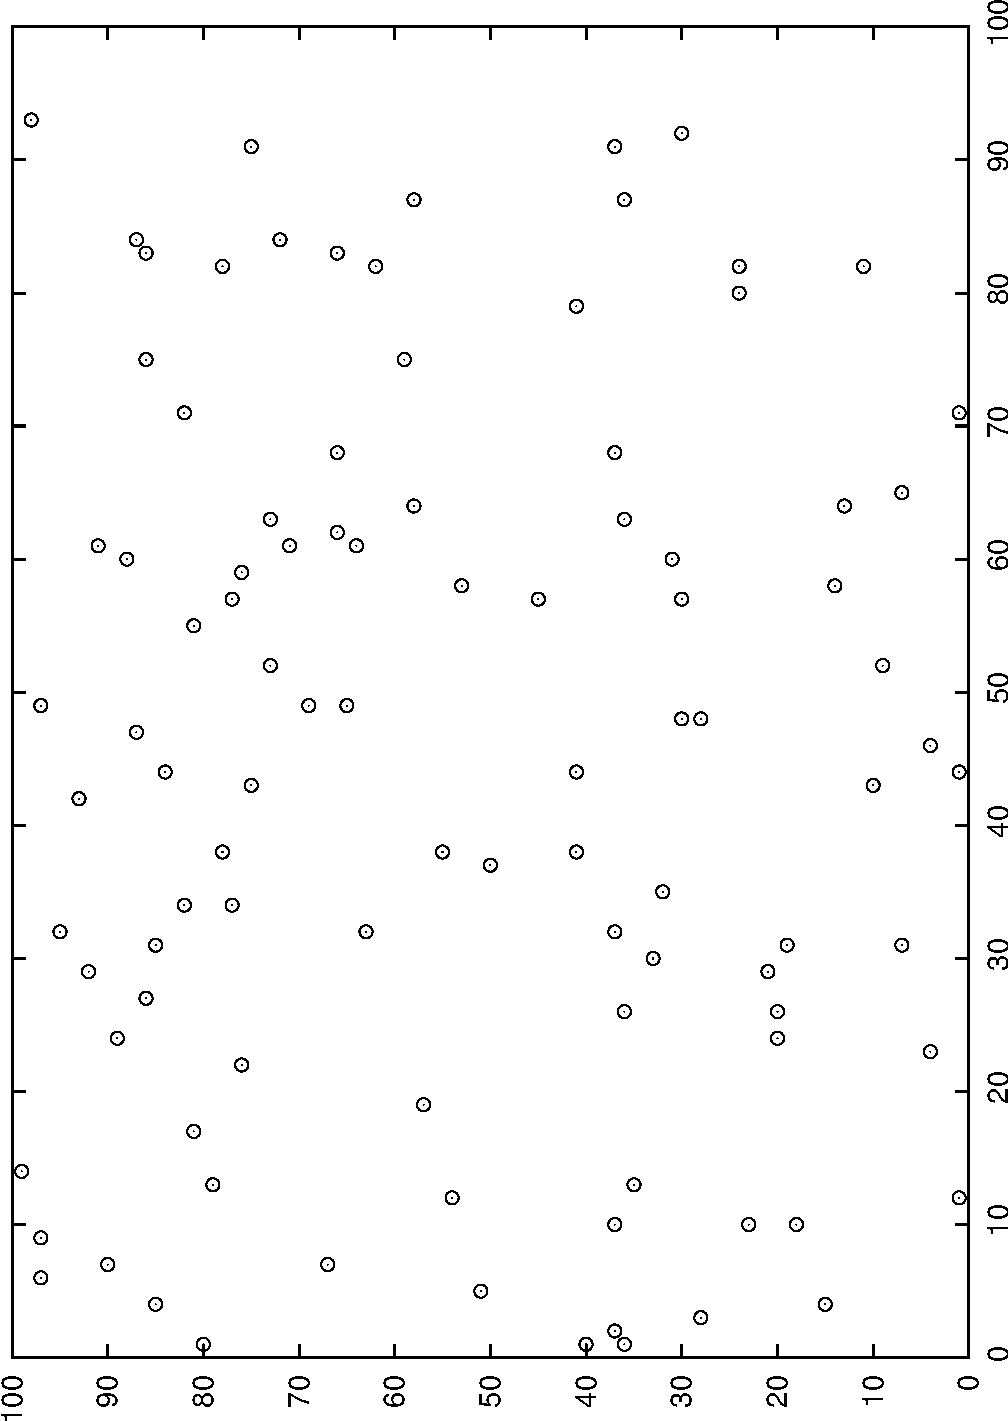
\includegraphics[%
  width=8cm,
  keepaspectratio]{figuras/exrandsparse}


\caption{\label{cap:exsparse}Elementos no nulos de una matriz sparse creada
con \texttt{sprand}}
\end{figure}


\begin{description}
\item [spdiags\index{spdiags}]Extrae e introduce diagonales en matrices
sparse.
\end{description}
Al igual que su función homóloga \texttt{diag} tiene un gran sentido
físico. De hecho tiene mucha mayor utilidad en la función de creación
\texttt{spdiags} que \texttt{diag} porque las matrices en banda entran
en la definición de matrices sparse. La única consideración a tener
en cuenta es que las matrices en banda se resuelven rápidamente de
manera exacta mediante una factorización LU diseñada para matrices
sparse. Utilizaremos los métodos iterativos con matrices que no cumplan
ningún patrón evidente o sencillo.


\subsubsection{Manipulación y operaciones con matrices sparse}

\begin{description}
\item [sphcat\index{sphcat}]Concatena horizontalmente dos matrices sparse
de dimensiones compatibles.
\item [spvcat\index{spvcat}]Concatena verticalmente dos matrices sparse
de dimensiones compatibles.
\item [spabs\index{spabs}]Calcula el valor absoluto de los elementos complejos
de una matriz sparse sin cambiar el carácter de la misma.
\item [spreal\index{spreal}]Calcula la parte real de los elementos complejos
de una matriz sparse sin cambiar el carácter de la misma.
\item [spimag\index{spimag}]Calcula la parte imaginaria de los elementos
de una matriz sparse sin cambiar el carácter de la misma.
\item [spinv\index{spinv}]Calcula la matiz inversa de una matriz sparse.
\end{description}
Sin embargo no es recomendable que utilicemos \texttt{spinv} para
resolver sistemas de ecuaciones lineales. Como en el caso de sistemas
de ecuaciones en matrices convencionales es recomendable que optemos
por el operador \texttt{\textbackslash{}} para invertir la matriz
del sistema.


\subsection{Matrices tridiagonales (Octave)}

Son uno de los tipos de matrices más buscadas; tienen un gran sentido
físico (provienen de algunas ecuaciones en diferencias) y son muy
adecuadas para el cálculo numérico. Son un caso particular de matrices
sparse pero al ser tan sencillas pueden resolverse directamente sin
realizar demasiados cálculos. La función de resolución de sistemas
de ecuaciones con una matriz tridiagonal es \texttt{trisolve\index{trisolve}.}


\subsection{Matrices no regulares.}

Una de las características más importantes del operador \
es que también sirve en el caso de tener un sistema con exceso o defecto
de ecuaciones. El operador ya no calcula la matriz inversa sino que
busca una solución cuyo error cumple la condición de la norma mínima
o busca el subespacio solución. En este caso se dice que en vez de
buscar la inversa se calcula una pseudoinversa que resuelve la ecuación.
El tratamiento de este tipo de problemas suele omitirse en la mayoría
de cursos de álgebra en ingeniería, sin embargo tiene una gran utilidad
en cálculo numérico y es una herramienta relativamente importante.
Creo que no es en vano si intentamos entender con un poco más de profundidad
el tratamiento de estas aplicaciones lineales sin entrar en formalismos.


\subsubsection{Singular Value Decomposition (SVD)}

Se demuestra que cualquier matriz de aplicación lineal acepta una
descomposición del tipo:\[ A=UwV^{\top}\] donde $U$ y $V^{\top}$ son
matrices ortogonales y $w$ una matriz diagonal que contiene los
valores singulares. Las matrices ortogonales, o más concretamente las
matrices de una transformación ortogonal, tienen la propiedad de
mantener los ángulos en la transformación.  Las matrices de giro son
un ejemplo de transformación ortogonal. La matriz $w$, al ser
diagonal, no produce ningún tipo de rotación, simplemente expande o
contrae determinadas direcciones. La demostración de la existencia de
esta descomposición va mucho más allá de los objetivos de este libro.
Se utiliza la notación $V^{\top}$ para esta matriz debido a que para
cumplir la definición de matiz de transformación ortogonal sus
columnas deben ser vectores ortogonales; es sólo un formalismo porque
se demuestra también que la inversa de una transformación ortogonal es
también una transformación ortogonal y es equivalente a su traspuesta.
Ayuda escribir la anterior ecuación especificando las dimensiones:
$$
A_{(N\times M)}=U_{(N\times M)}w_{(M\times M)}V_{(M\times M)}^{\top}$$
Vemos también que las dimensiones son correctas, aplicando que
$V^{\top}\equiv V^{-1}$:
$$ A_{(N\times M)}V_{(M\times M)}=U_{(N\times
  M)}w_{(M\times M)}$$


Ahora, un repaso de álgebra de parte de \cite{Algebra}. Si nuestra
matriz $A$ es la matriz de una aplicación lineal \[ f:S\longrightarrow
T\] podemos definir dos subespacios en $S$; el Núcleo, subespacio que
forman los vectores que tienen al vector nulo como imagen y el
subespacio Imagen que es el subespacio $f(S)$de $T$. Por ejemplo, sean
$S$ y $T$ los siguientes espacios reales:

\begin{itemize}
\item $S$ son las funciones polinómicas $p(x)=a+bx+cx^{2}+dx^{3}$
\item $T$ el espacio de funciones de $\mathbb{R}$ en $\mathbb{R}$
\end{itemize}
Consideremos la aplicación lineal de $f:S\longrightarrow T$ definida
por $f(p(x))=p^{\prime}(x)$, la derivada según la variable
independiente; o sea: $f(a+bx+cx^{2}+dx^{3})=b+2cx+3dx^{2}$. La imagen
de $f$ es el subespacio de $T$ formado por los polinomios de grado
menor o igual que 2. El núcleo de $f$ es el subespacio de $T$ que
forman los polinomios constantes.

Si volvemos a la forma de la descomposición propuesta por la SVD,
$$
A_{(N\times M)}=U_{(N\times M)}w_{(M\times M)}V_{(M\times M)}^{\top}$$

Tomemos la condición de $N<M$, es decir, un sistema con menos
ecuaciones que incógnitas. En este caso la aplicación lineal será
$f:\mathbb{R}^{M}\longrightarrow\mathbb{R}^{N}$, si ninguna de las
filas es combinación lineal del resto tendremos una imagen de
dimensión $N$ y un núcleo de dimensión $M-N$. Se cumple además que la
cantidad de valores singulares no nulos será $N$ y que las $M-N$
columnas asociadas a los valores singulares nulos formarán la base del
núcleo. La demostración de lo anterior está también fuera de los
objetivos de este libro.

Esta operación es perfectamente válida también para el caso $N>M$ en
el que tenemos más ecuaciones que incógnitas.

Para obtener las tres matrices de la descomposición Matlab proporciona
la siguiente función

\begin{description}
\item [svd\index{svd}]Descomposición en valores singulares. Si se pide
  únicamente un valor de salida retorna un vector con valores
  singulares.  Con tres valores de salida retorna la descomposición
  matricial completa.
\end{description}
Para ejemplificar el uso de la ecuación vamos a intentar descomponer
en valores singulares la ya clásica matriz...

  \begin{verbatim}
octave:3> a=[1,2,3;4,5,6;7,8,9];
octave:4> [U,w,V]=svd(a)
U =
  -0.21484   0.88723   0.40825
  -0.52059   0.24964  -0.81650
  -0.82634  -0.38794   0.40825
w =
  16.84810   0.00000   0.00000
   0.00000   1.06837   0.00000
   0.00000   0.00000   0.00000
V =
  -0.479671  -0.776691  -0.408248
  -0.572368  -0.075686   0.816497
  -0.665064   0.625318  -0.408248
\end{verbatim}
Efectivamente, uno de los valores singulares es nulo debido a que la
matriz es singular. Para analizar más en profundidad las matrices,
Matlab proporciona además las siguientes funciones:

\begin{description}
\item [rank\index{rank}]Calcula el rango de la matriz, es decir, el
  número de valores singulares no nulos o la dimensión de la imagen de
  la aplicación.
\item [null\index{null}]Calcula la dimensión del núcleo de una
  aplicación lineal expresada por una matriz, esto es, el número de
  valores singulares nulos.
\end{description}

\subsubsection{Problemas con defecto o exceso de ecuaciones.}

Si lo único que nos interesa es resolver $\mathbf{a}x=b$... ¿Qué
calcula exactamente el operador \texttt{\textbackslash{}} cuando $N<M$?
Lo que hace es calcular la pseudoinversa a partir de la descomposición
en valores singulares. La fórmula de la pseudoinversa es la siguiente:
$$A^{+}=Vw^{-1}U^{\top}$$
Esta matriz da una solución al problema del tipo:
$$x=a^{+}b+v$$
donde $v$ es una combinación lineal cualquiera de vectores del núcleo
definido por la matriz $\mathbf{a}$. Se demuestra que la solución
que minimiza la norma del error $r\equiv|\mathbf{a}x-b|$ (mínimos
cuadrados) es precisamente la que cumple $v=0$. Acabamos de deducir
la forma de cualquier solución hallada por el método de los mínimos
cuadrados.

En el apartado \ref{sub:=BFQu=E9-calcula-el} analizaremos las propiedades
de la SVD en el cálculo de ajustes polinómicos de series de datos.


\section{Autovalores}

\begin{description}
\item [eig\index{eig}]Calcula los autovalores y autovectores de una matriz
cuadrada.
\end{description}
